\chapter{Profil Mitra Industri}
\begin{figure}[!htb]
    \centering
    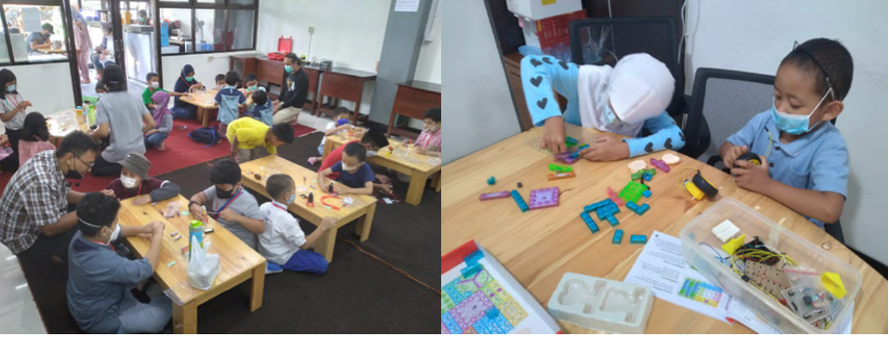
\includegraphics[width=0.7\textwidth]{figures/KegiatanKiddo.png}
    \caption{Kegiatan di Kido Robot}
    \label{fig:kegiatankiddo}
\end{figure}
\begin{figure}[!htb]
    \centering
    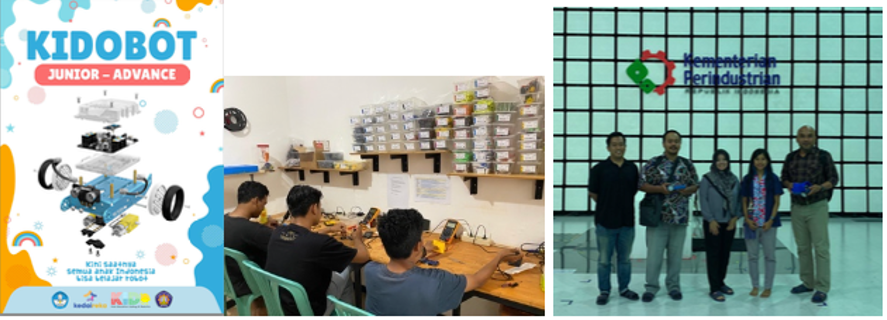
\includegraphics[width=0.7\textwidth]{figures/ProdukWorkshopKiddo.png}
    \caption{Produk dan Workshop di Kido Robot}
    \label{fig:produkkiddo}
\end{figure}
Kido Robot adalah perusahaan yang berfokus pada produksi dan pelatihan modul edukasi robotika. Inisiatif Kido Robot yang dimulai sejak 2014, memiliki misi untuk menyiapkan sumber daya manusia dalam menghadapi ekonomi digital, khususnya di bidang teknologi robotika. Antara lain dengan melakukan pelatihan private, kursus rutin grup dan workshop robotik. Kido Robot juga berkolaborasi dengan sekolah-sekolah dan ikatan guru dalam pengembangan dan pelatihan robotika. Gambar~\ref{fig:kegiatankiddo}  adalah gambaran kegiatan di Kiddo Robot. Gambar~\ref{fig:produkkiddo} adalah gambaran salah satu produk, situasi workshop dan kerjasama yang pernah dilakukan dengan Politeknik Negeri Malang. 

Dedikasi bahwa platform pendidikan dalam aliran berkelanjutan dari fase prasekolah ke fase dewasa harus disediakan untuk kreativitas dan daya pikir mengembangkan pendidikan yang akan menjadi dasar untuk menumbuhkan bakat di setiap bidang, Kido Robot memfasilitasi berbagai platform pendidikan untuk segala usia. Khususnya, alat pendidikan berkualitas baik untuk robot, pengkodean, dan STEM memungkinkan pembelajaran bakat yang efektif. 

Kido Robot telah banyak bekerja sama dengan sekolah-sekolah di area Kota Malang, diantaranya sekolah Andalusia Kids, Tweddle Land, Al Muttaqien, dan lain sebagainya. Tidak hanya dalam kegiatan ekstrakulikuler saja namun dalam berkolaborasi membuat modul belajar robotika juga. Sehingga dapat tercipta modul-modul edukasi yang baik. Selain bekerja sama dengan sekolah, Kido Robot juga menjalin kerjasama kegiatan dengan taman atau lokasi permainan anak. Misi yang dicapai adalah bukan hanya untuk menjadikan siswa-siswa menjadi juara, tapi lebih daripada hal tersebut adalah membuat siswa-siswa senang belajar utamanya dalam hal teknologi dan membuat mereka siap dalam menghadapi perkembangan teknologi yang signifikan. 
